\chapter{Практическая часть}

\section{Задание \No{}1}
Представления списков, указанных в условии данной лабораторной работы, в виде списочных ячеек изображены на рисунках 2.1-2.6.

\begin{enumerate}
    \item '(open close halph)
        \begin{figure}[H]
            \centering
            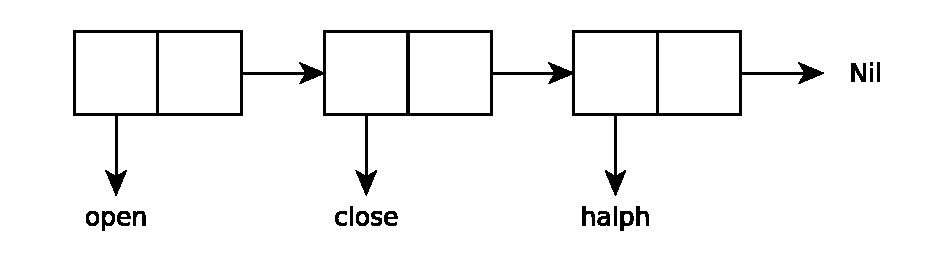
\includegraphics[scale=0.60]{data/pdf/01-01.pdf}
            \caption{Список '(open close halph)}
        \end{figure}
    \item '((TOOL) (call))
        \begin{figure}[H]
            \centering
            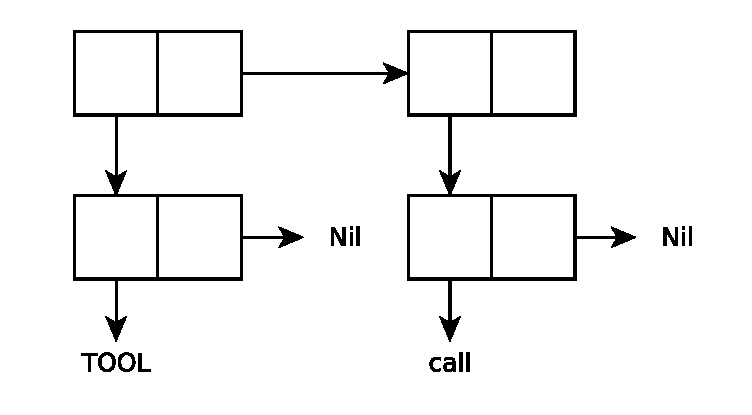
\includegraphics[scale=0.60]{data/pdf/01-02.pdf}
            \caption{Список '((TOOL) (call))}
        \end{figure}
    \item '((open1) (close2) (halph3))
        \begin{figure}[H]
            \centering
            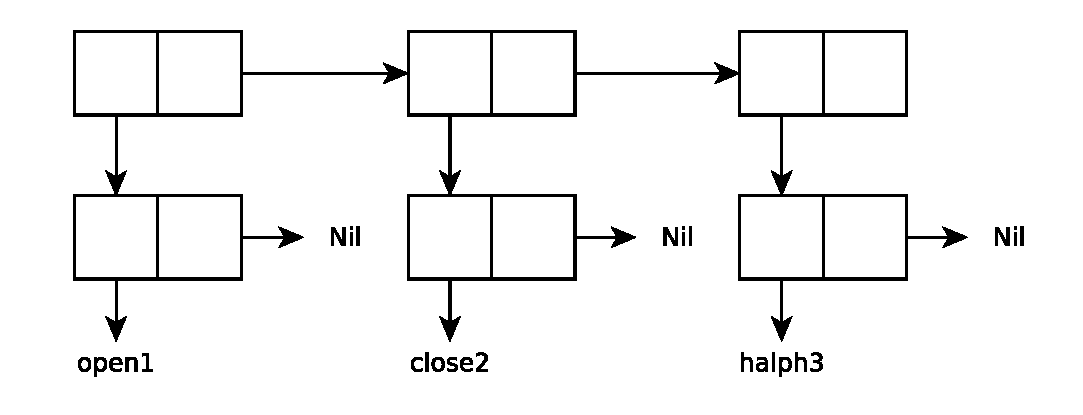
\includegraphics[scale=0.60]{data/pdf/01-03.pdf}
            \caption{Список '((open1) (close2) (halph3))}
        \end{figure}
    \item '((TOOL1) ((call2)) ((sell)))
        \begin{figure}[H]
            \centering
            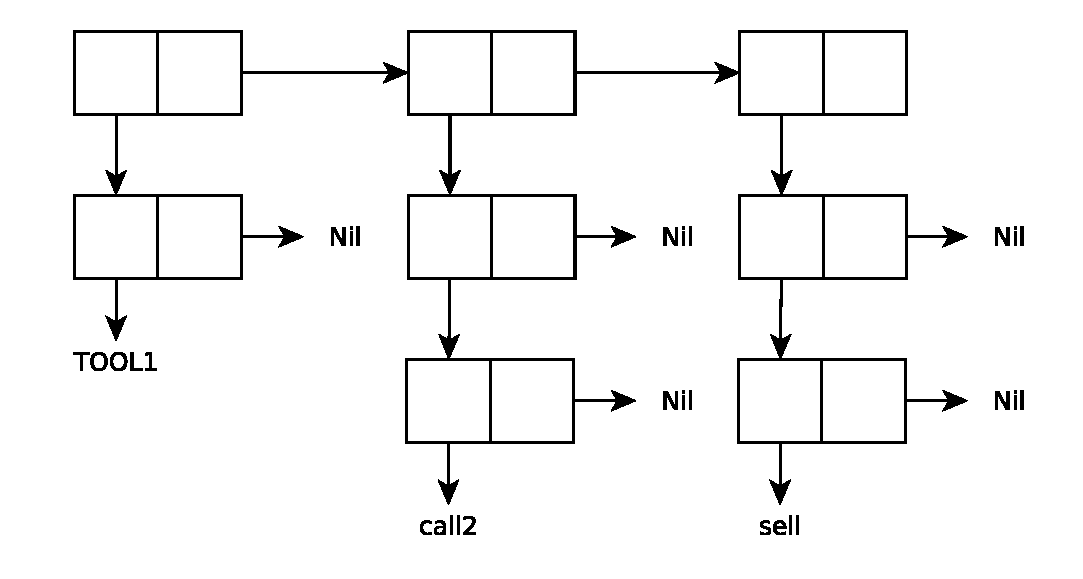
\includegraphics[scale=0.60]{data/pdf/01-04.pdf}
            \caption{Список '((TOOL1) ((call2)) ((sell)))}
        \end{figure}
    \item '(((TOOL) (call)) ((sell)))
        \begin{figure}[H]
            \centering
            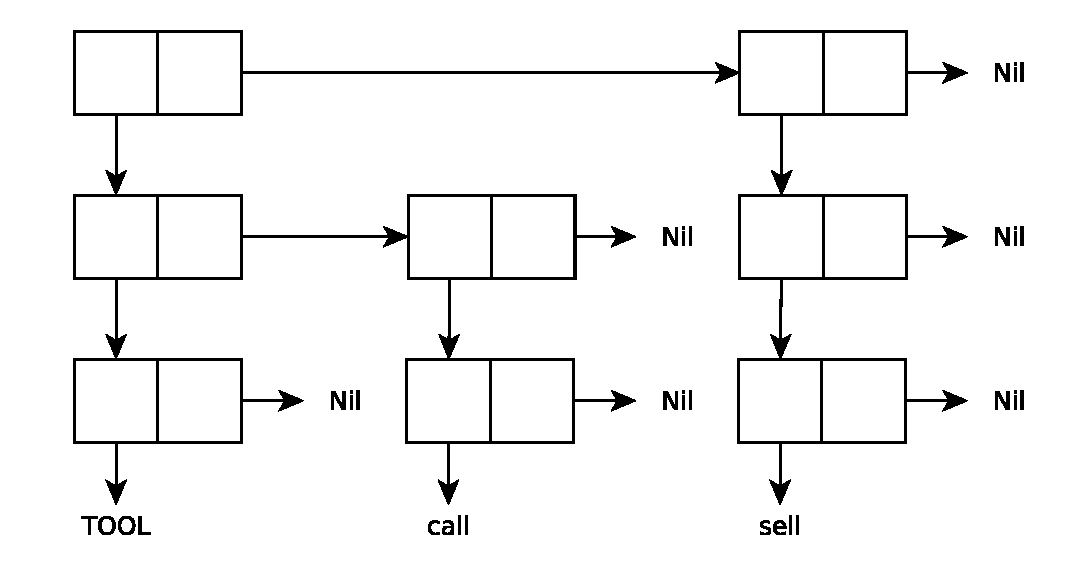
\includegraphics[scale=0.60]{data/pdf/01-05.pdf}
            \caption{Список '(((TOOL) (call)) ((sell)))}
        \end{figure}
    \item '((one) for all (and (me (for you))))
        \begin{figure}[H]
            \centering
            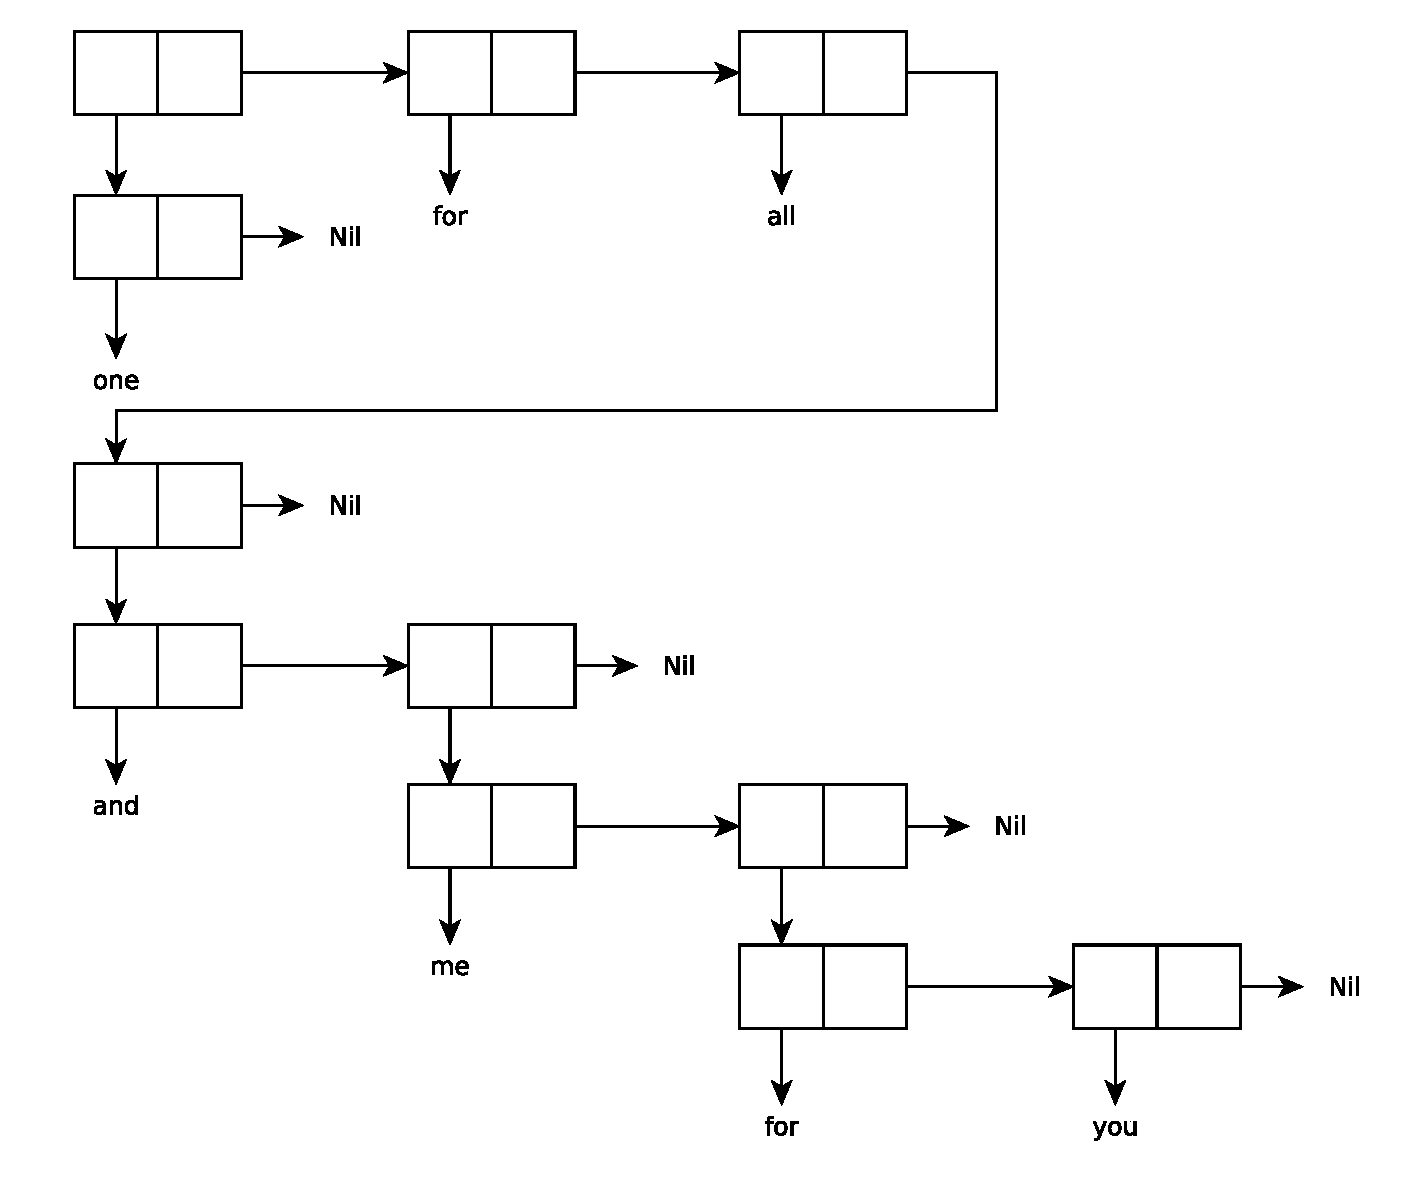
\includegraphics[scale=0.60]{data/pdf/01-06.pdf}
            \caption{Список '((one) for all (and (me (for you))))}
        \end{figure}
\end{enumerate}

\section{Задание \No{}2}

В листинге 2.1 приведены три выражения на языке Lisp, которые возвращают второй, третий и четвёртый элементы списков. Для этого были использованы функции доступа car и cdr. Функция \textbf{car} возвращает голову списка, а \textbf{cdr} - его хвост. Результаты выражений приведены в комментариях под соответствующим им строкам.

\lstset{language=lisp}
\begin{lstlisting}[caption={Выражения, возвращающие 2, 3 и 4 элементы списка}]
(car (cdr '((4) (8 2 2) (1 (4 (1 (4)))) 1 (6 2))))
; (8 2 2)

(car (cdr (cdr '((3 2 1) (3) (8 8 0) (0 5 5 (5 3 (5))) 3 5))))
; (8 8 0)

(car (cdr (cdr (cdr '(1 (2 2) ((3) (3 3)) (4 4 (4 (4))) 5)))))
; (4 4 (4 (4)))
\end{lstlisting}

(car (car (cdr (cdr (cdr '((one) for all (and (me (for you)))))))))
